%
% This is the LaTeX template file for lecture notes for CS294-8,
% Computational Biology for Computer Scientists.  When preparing 
% LaTeX notes for this class, please use this template.
%
% To familiarize yourself with this template, the body contains
% some examples of its use.  Look them over.  Then you can
% run LaTeX on this file.  After you have LaTeXed this file then
% you can look over the result either by printing it out with
% dvips or using xdvi.
%
% This template is based on the template for Prof. Sinclair's CS 270.

\documentclass[twoside]{article}
\usepackage{graphics}
\usepackage{amsmath}
\usepackage{amssymb}
\usepackage{hyperref}
\usepackage{IEEEtrantools}
\usepackage{graphicx}
\usepackage{float}

\setlength{\oddsidemargin}{0.25 in}
\setlength{\evensidemargin}{-0.25 in}
\setlength{\topmargin}{-0.6 in}
\setlength{\textwidth}{6.5 in}
\setlength{\textheight}{8.5 in}
\setlength{\headsep}{0.75 in}
\setlength{\parindent}{0 in}
\setlength{\parskip}{0.1 in}
\usepackage[makeroom]{cancel}
%
% The following commands set up the lecnum (lecture number)
% counter and make various numbering schemes work relative
% to the lecture number.
%
\newcounter{lecnum}
\renewcommand{\thepage}{\thelecnum-\arabic{page}}
\renewcommand{\thesection}{\thelecnum.\arabic{section}}
\renewcommand{\theequation}{\thelecnum.\arabic{equation}}
\renewcommand{\thefigure}{\thelecnum.\arabic{figure}}
\renewcommand{\thetable}{\thelecnum.\arabic{table}}

%
% The following macro is used to generate the header.
%
\newcommand{\lecture}[5]{
   \pagestyle{myheadings}
   \thispagestyle{plain}
   \newpage
   \setcounter{lecnum}{#1}
   \setcounter{page}{1}
   \noindent
   \begin{center}
   \framebox{
      \vbox{\vspace{2mm}
    \hbox to 6.28in { {\bf CMPUT 652: Reinforcement Learning with Robots
                        \hfill Fall 2019} }
       \vspace{4mm}
       \hbox to 6.28in { {\Large \hfill Lecture #1: #2  \hfill} }
       \vspace{2mm}
       \hbox to 6.28in { {\it Instructor: #3 \hfill Scribe: #4} }
      \vspace{2mm}}
   }
   \end{center}
   \markboth{Lecture #1: #2}{Lecture #1: #2}
   {\bf Disclaimer}: {\it These notes have not been subjected to the
   usual scrutiny reserved for formal publications.  They may be distributed
   outside this class only with the permission of the Instructor.}
   \vspace*{4mm}
}

%
% Convention for citations is authors' initials followed by the year.
% For example, to cite a paper by Leighton and Maggs you would type
% \cite{LM89}, and to cite a paper by Strassen you would type \cite{S69}.
% (To avoid bibliography problems, for now we redefine the \cite command.)
% Also commands that create a suitable format for the reference list.

%% This has been commented by Dhawal
% \renewcommand{\cite}[1]{[#1]}
% \def\beginrefs{\begin{list}%
%         {[\arabic{equation}]}{\usecounter{equation}
%          \setlength{\leftmargin}{2.0truecm}\setlength{\labelsep}{0.4truecm}%
%          \setlength{\labelwidth}{1.6truecm}}}
% \def\endrefs{\end{list}}
% \def\bibentry#1{\item[\hbox{[#1]}]}

%Use this command for a figure; it puts a figure in wherever you want it.
%usage: \fig{NUMBER}{SPACE-IN-INCHES}{CAPTION}
\newcommand{\fig}[3]{
			\vspace{#2}
			\begin{center}
			Figure \thelecnum.#1:~#3
			\end{center}
	}
% Use these for theorems, lemmas, proofs, etc.
\newtheorem{theorem}{Theorem}[lecnum]
\newtheorem{lemma}[theorem]{Lemma}
\newtheorem{proposition}[theorem]{Proposition}
\newtheorem{claim}[theorem]{Claim}
\newtheorem{corollary}[theorem]{Corollary}
\newtheorem{definition}[theorem]{Definition}
\newenvironment{proof}{{\bf Proof:}}{\hfill\rule{2mm}{2mm}}

% **** IF YOU WANT TO DEFINE ADDITIONAL MACROS FOR YOURSELF, PUT THEM HERE:

%%===========================================================================
%% defining the expectation operator
%%---------------------------------------------------------------------------
\DeclareMathOperator{\E}{\mathbb{E}}
\DeclareMathOperator{\Real}{\mathbb{R}}
\DeclareMathOperator{\real}{\mathbb{R}}
\DeclareMathOperator{\xvec}{\textbf{x}}

\DeclareMathOperator*{\argmax}{argmax} % thin space, limits underneath in displays

% \DeclareMathOperator{\thetagd}{\theta^{GD}}
% \DeclareMathOperator{\rv}{X} % define random variable 
% \DeclareMathOperator{\sc}{} %
% \DeclareMathOperator{}{} %
% \DeclareMathOperator{}{} %
% \DeclareMathOperator{}{} %

% \DeclareMathOperator{}{}
%%===========================================================================

\begin{document}
%FILL IN THE RIGHT INFO.
%\lecture{**LECTURE-NUMBER**}{**DATE**}{**LECTURER**}{**SCRIBE**}
\lecture{5}{September 17}{Rupam Mahmood}{Matthew McLeod}
%\footnotetext{These notes are partially based on those of Nigel Mansell.}

% **** YOUR NOTES GO HERE:

% Some general latex examples and examples making use of the
% macros follow.  
%**** IN GENERAL, BE BRIEF. LONG SCRIBE NOTES, NO MATTER HOW WELL WRITTEN,
%**** ARE NEVER READ BY ANYBODY.


\section{Discussion Last Lecture}
In the previous lecture, we covered the difference between exact and sampled based MSE as well as the optimization for both of these cases. 

\section*{Course Administration}
%do you expect summary of previous week?

The following is a summary of the course administration component of the beginning of class.

For the final project, you will be working with a robot. There are 3 available types: the UR5 arm, iRobot Create 2s, and a collection of Dynamixel servomotors. 
\begin{itemize}
    \item There is one available UR5 arm from Kindred Inc.
    \item A show of hands was done for people interested in working with iRobot Create 2s.
    \item A collection of smaller robotic components that could be assembled to do a task.
\end{itemize}

It is possible to try working with a robot not listed here, but extensive research is required to ensure that it will be appropriate and feasible for the course. Talk to professor Mahmood should you have questions about this.
In order to determine who works with which robot, priority will be given to those who have the highest assignment grades up until that point.

\section{Bandits}
The k-armed bandits problem refers to having multiple actions associated with a reward distribution. There are additional complications that can be added to the bandits problem such as contextual bandits. Contextual bandits is when there are different reward distribution per action conditioned on a stimulus being shown to the agent. However, in the remaining of the lecture, we will not consider contextual bandits and remain in the k-armed bandit setting.

\section{Policies}
Policies are a key component in understanding how an agent should act in a bandits scenario. A policy is a function that takes in an action as input and outputs the probability of taking the action. A policy can either be deterministic or stochastic.

%The notation concerning policies are as follows:

A policy is defined as:
% \begin{align*}
    \begin{equation}
        \pi(a) = p(a) = P_\pi\{A = a\}
    \end{equation}
% \end{align*}
where, $a$ is the action and $\pi(a)$ is the probability of the action.

The value of taking action $a$ is the action-value function $q$ and is shown below:
\begin{equation}
    q(a) = \E[R|A=a]
\end{equation}
where $R$ is the reward. The optimal action to maximize reward is then:
\begin{equation}
    a^* = \argmax_a q(a)
\end{equation}
If you have a policy $\pi$ that follows the optimal actions, it is called an optimal policy and denoted with $\pi^*$. 
%It is common convention to add $a^*$ to a function when it is the optimal function.

In order to find the action-value function, stochastic gradient descent (SGD) can be used to reduce the MSE. Recall the form of SGD from the previous lecture. The update rule for SGD applied to $q(a)$ is shown below.
\begin{equation*}
    \hat{q}_{t+1}(A_t) = \hat{q}_t(A_t) + 2\alpha_t[R_t-\hat{q}_t(A_t)]
\end{equation*}
where, $\hat{q}$ is the incremental estimate of $q$,
$\alpha_t$ is step size applied to the error signal.

Remember that $\alpha$ has a large influence on how the function estimate is updated. A constant $\alpha$ exponentially weights more heavily recent error signals than older error signals. If $\alpha$ decays at a rate that is the inverse to the number of times the action has been, then all the error signals have been equally weighted.

\section{Analysis of Bandits}

Since bandits can occur in different environments and reward systems, it is useful to consider each combination individually. Table \ref{fig:just-alpha} shows the optimal $\alpha$ values for the different settings.

\begin{figure}[H]
  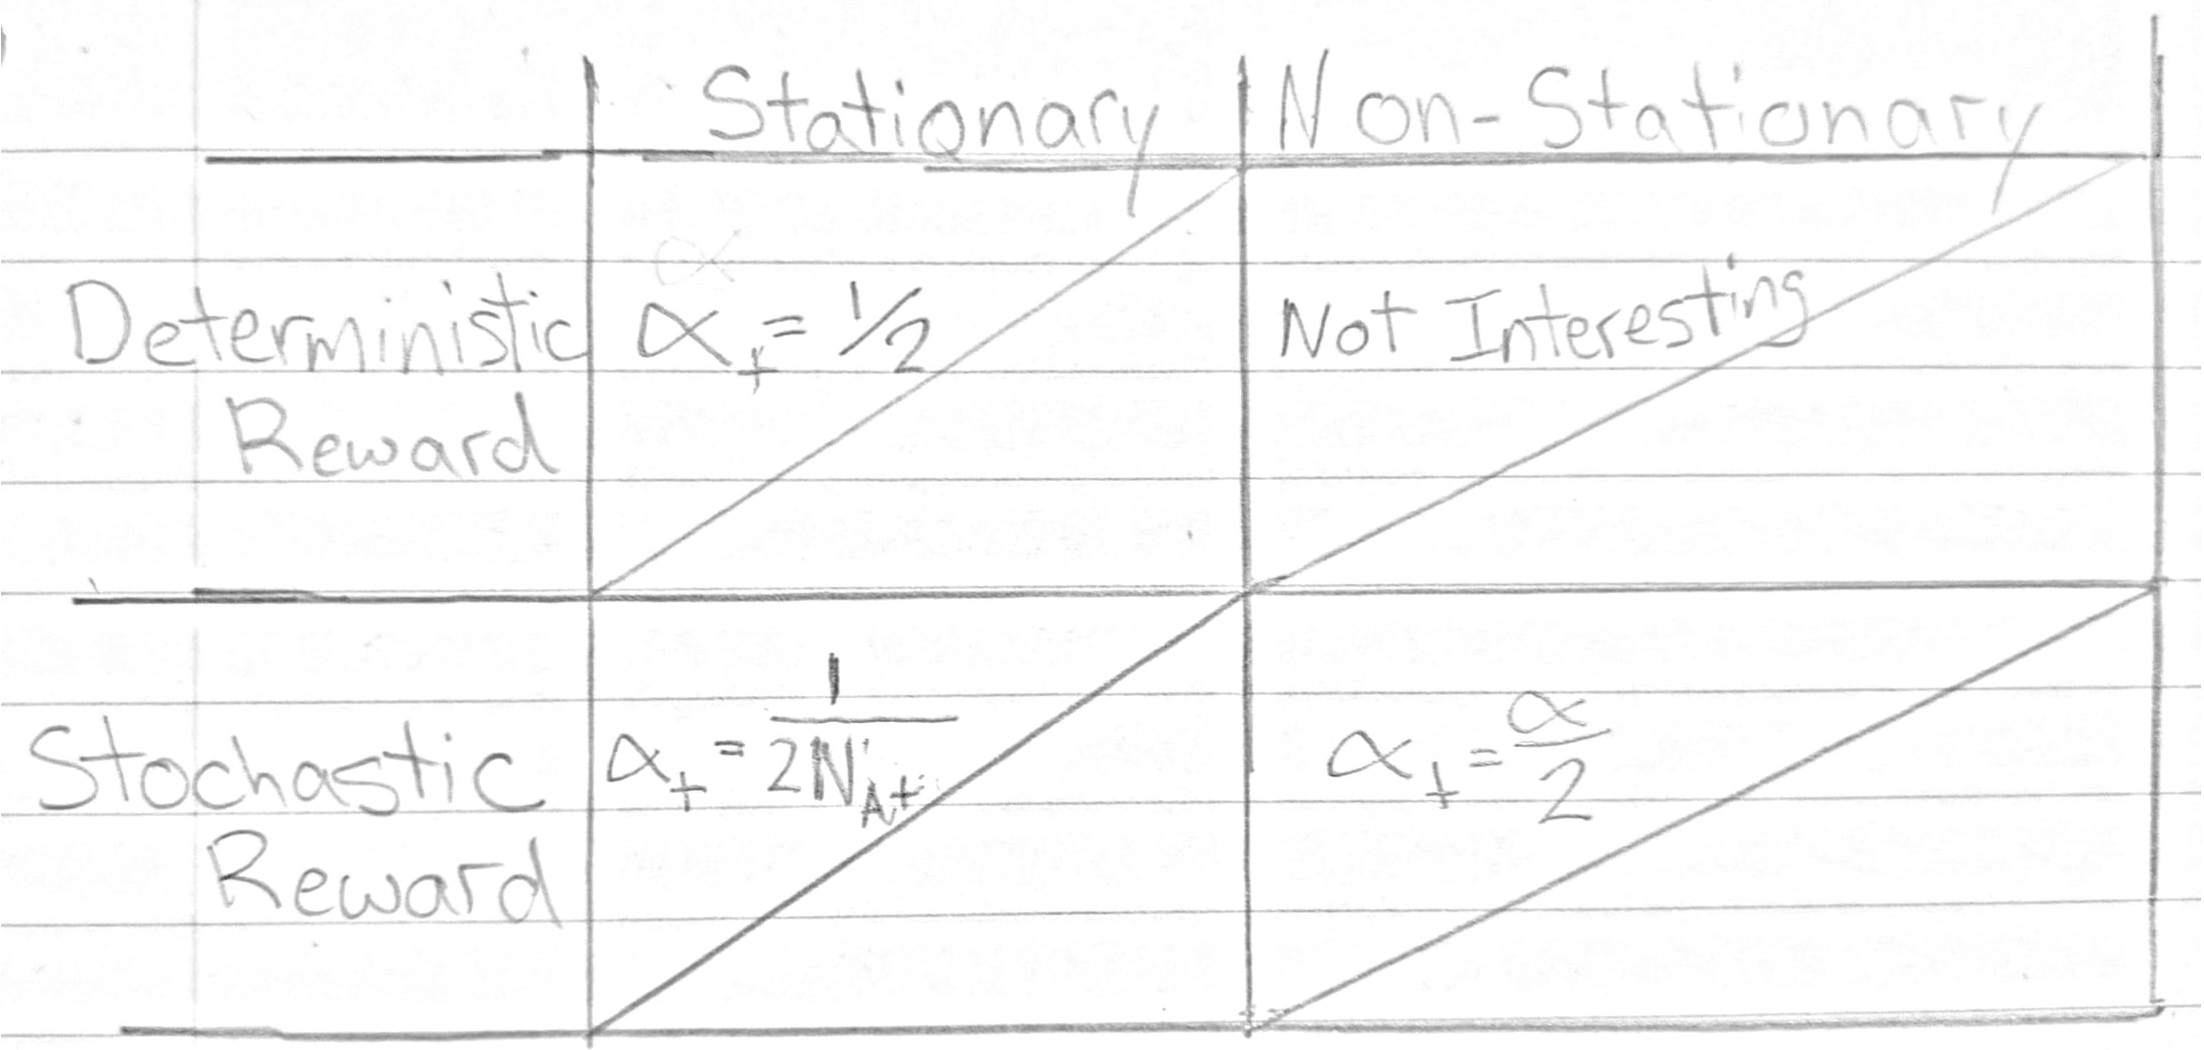
\includegraphics[scale=0.35]{alpha.jpg}
  \caption{The optimal $\alpha_t$ for different environments and reward structures.}
  \label{fig:just-alpha}
\end{figure}

Stationary means that the reward distribution never changes. Non-stationary means that the reward distribution may shift as the agent interacts with the environment. This may result in non-optimal actions becoming optimal. A deterministic reward is when the agent will always receive the same reward for a given action while stochastic reward means that the reward is being sampled from a distribution (excluding distributions like Dirac).

For the case of a stationary environment with a deterministic reward , it is best to have $\alpha_t = \frac{1}{2}$ so that the estimate of $q$ only relies on the previous reward. This allows the estimate to immediately jump to the correct reward estimate from only a single trial. If the reward signal changes to a stochastic reward, then it is best to let $\alpha_t$ be equal to $\frac{1}{2N_{A_t}}$ where $N_{A_t}$ is the number of times action $A_t$ has been chosen. This allows the agent to equally weight all sampled rewards and converge towards the true expected reward per action.

For the non-stationary case, a deterministic reward is not interesting since the reward is changing and essentially is a non-stationary stochastic reward. For the case of a non-stationary stochastic reward, $\alpha_t$ can be set to a constant to track in response to each sample at the same rate. By having $\alpha_t$ set to a constant, it allows the agent to exponentially weight the rewards and thus `forget' the older ones. This enables more effective tracking of the moving distribution of rewards. 

There is also a problem of exploration versus exploitation in the bandits problem.  It does not matter what $\alpha$ value the agent has for an action if the action is never chosen. It is also important that the agent samples enough times each action to get an accurate estimate of the reward for the action. One solution is the $\epsilon$-\emph{greedy} method where $\epsilon \in [0,1]$. The agent acts optimally (also called greedily) with a probability of $1-\epsilon$, and the agent acts randomly with $\epsilon$ probability. Table \ref{fig:full} shows reasonable $\epsilon$ values for each scenario as well.

\begin{figure}[H]
  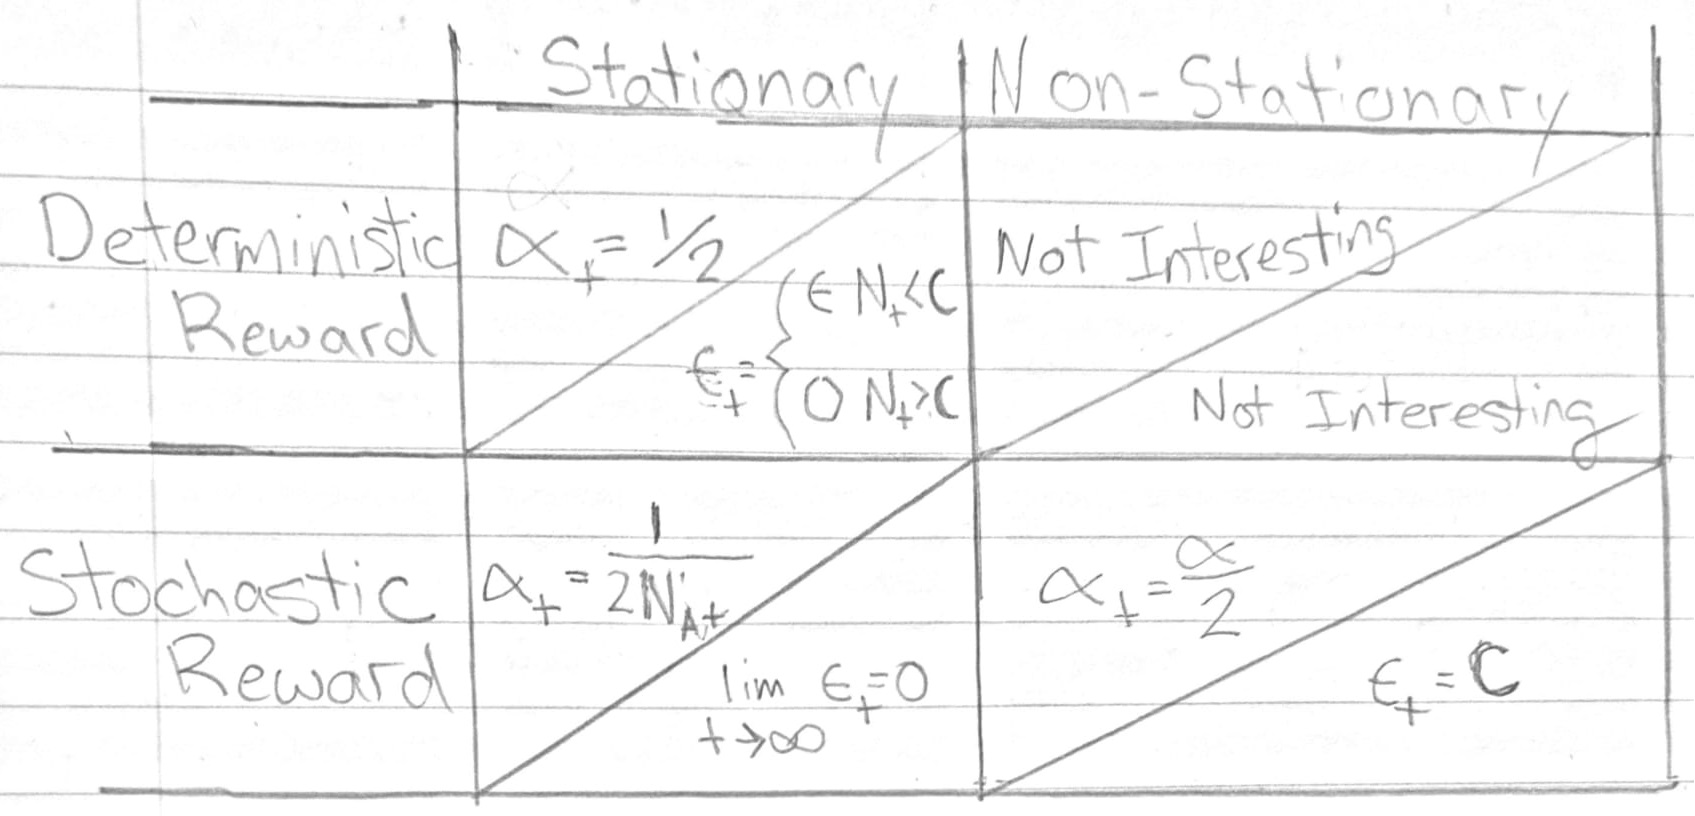
\includegraphics[scale=0.4]{full.jpg}
  \caption{The optimal $\alpha_t$ and $\epsilon_t$ for different environments and reward structures.}
  \label{fig:full}
\end{figure}

For the stationary environment with a deterministic reward, $\epsilon_t$ should explore every action. Once every action has been tried atleast once, then $\epsilon$ should be 0 as this allows full exploitation. Since the environment is stationary, the optimal action will always be the same. When the reward signal is stochastic, then a decreasing $\epsilon$ is ideal and converges towards 0 as the action-value function converges towards the true expected value of the optimal action. 

For similar reasons to table \ref{fig:just-alpha}, the non-stationary deterministic reward is not interesting. For a stochastic reward, $\epsilon$ should be a constant value. This allows continual exploration that enables the discovery of shifting optimal actions as the reward distributions change.


\section{Policy Gradient Methods}
The action-value function is useful for cases of a finite and discrete number of actions such as the bandit setting analyzed thus far. However, when the action space is continuous relying on value functions becomes difficult. To act optimally, one must take the max out of the set of actions. This becomes difficult to do in continuous domains. Therefore, policy gradient methods are an alternative which alleviate this problem.

If the objective function for the discrete case is:
\begin{equation}
    \mathcal{V}(\theta) = \E[q_\theta(A_t)] = \sum_{a\in\mathcal{A}} \pi_\theta(a) q(a),
\end{equation}
then for the continuous case:
\begin{equation}
    \mathcal{V}(\theta) = \int_{\mathcal{A}} \pi_\theta(a)q(a)da
\end{equation}
To maximize the objective function, take the derivative with respect to the parameterization of $\theta$. Since we want to typically minimizing functions as this is the more common paradigm in optimization, we can multiply the function by $-1$.

\begin{equation}
    \begin{split}
    \nabla_\theta\mathcal{V}(\theta) = -\int  \nabla_\theta\pi_\theta(a)q(a)da \\ 
    \nabla_\theta\mathcal{V}(\theta) = -\int  \pi_\theta(a)\frac{\nabla_\theta\pi_\theta(a)}{\pi_\theta(a)}q(a)da \\
    \nabla_\theta\mathcal{V}(\theta) = -\int  \pi_\theta(a)\nabla_\theta \log\pi_\theta(a)q(a)da
    \\
    \nabla_\theta\mathcal{V}(\theta) = -\E[\nabla_\theta \log\pi_\theta(A_t)R_t]
    \end{split}
\end{equation}

Therefore, to apply this in stochastic gradient descent:

\begin{equation}
    \begin{split}
        \theta_{t+1} = \theta_t - \alpha_t\nabla \ell_t \\
        \theta_{t+1} = \theta_t + \alpha_t\nabla_\theta \log\pi_\theta(A_t)R_t.
    \end{split}
\end{equation}

\section{Fundamental Difference between Supervised Learning and Reinforcement Learning}

At this point, it is reasonable to wonder what is the difference between supervised learning and reinforcement learning. The table below shows the comparison of the supervised learning dataset of MNIST and a contextual bandits scenario.

\begin{table}[H]
\begin{tabular}{|l|l|l|}
\hline
Example Environments & MNIST       & contextual Bandits \\ \hline
Input                & Image: \textbf{X}    & Context: \textbf{X}      \\ \hline
Processing Output    & Prediction: $f_\theta(\textbf{X})$ & Action: $f_\theta(\textbf{X})$          \\ \hline
Corrective Signal    & True Label: Y  & Reward: R          \\ \hline
\end{tabular}
\end{table}

The true difference relies on the fact that the agent is interacting and influencing the environment. Both methods fall into function approximation, but in reinforcement learning the mind of the agent is important as it effects future events.

\section{Cross Entropy Relationship to MSE}

Recall that maximizing the log likelihood results in finding the MSE solution for supervised regression under the assumption that the target values are distributed normally. For the sample based method, we want to minimize:
\begin{equation}
    \label{eq:sample-MSE}
 -  \frac{1}{t}\sum_{i=1}^{t}\log(p(Y_i|\theta,X_i).
\end{equation}

Cross entropy is defined as:

\begin{equation}
    \label{eq:cross-entropy}
    \begin{split}
        = -\int p^*(y)\log[p_\theta(y)dy] \\
        = -\E[\log p_\theta(y)]
    \end{split}
\end{equation}

The cross entropy shown in equation \ref{eq:cross-entropy} is the expected version of the sample based log-likelihood objective shown in equation \ref{eq:sample-MSE}. 
And from a function approximation perspective, cross-entropy objective, that is, trying to match the underlying distribution with a parameterized function, also makes sense.
Therefore, minimizing the cross entropy can be seen as a more fundamental objective, from which MSE can be derived.

\end{document}
